\documentclass[aspectratio=169,13pt,t] {beamer}
%
% Choose how your presentation looks.
%
% For more themes, color themes and font themes, see:
% http://deic.uab.es/~iblanes/beamer_gallery/index_by_theme.html
%
\mode<presentation>
{
  \usetheme{Madrid}      % or try Darmstadt, Madrid, Warsaw, ...
  \usecolortheme{beaver} % or try albatross, beaver, crane, ...
  \usefonttheme{serif}  % or try serif, structurebold, ...
%  \setbeamertemplate{navigation symbols}{}
  \setbeamertemplate{caption}[numbered]
  \setbeamertemplate{items}[default]
}

\usepackage[,UTF8,linespread=1.2]{ctex}
\usepackage{wrapfig}
\usepackage{caption}
\captionsetup[figure]{name=图,labelsep=period}
\usepackage[,most]{tcolorbox}
\usepackage{picinpar}


\usepackage{xcolor}
\definecolor{xy_blue}{cmyk}{0.6,0.35,0.0,0.4}
\definecolor{xy_orange}{cmyk}{0.0,0.7,1.0,0.0}
\definecolor{xy_green}{cmyk}{0.2,0.0,1.0,0.15}
\xdefinecolor{xy_gold}{RGB}{135,103,79}
\xdefinecolor{xy2_gold}{cmyk}{0,0.35,0.75,0.05}


\setbeamercolor{section number projected}{fg=red,bg=red!20}%控制球的颜色
\setbeamercolor{subsection number projected}{fg=blue,bg=blue!40}
\setbeamercolor{item}{fg=xy_gold} %设置列表项颜色

\usepackage{amsthm}
\newtheorem{peroration}{结论：}
\newtheorem{exploration}{探究：}
\newtheorem*{prooft}{证明：}
\newtheorem{question}{问题}
\newtheorem{exercise}{练习}
\newtheorem*{solve}{解:}
\newtheorem{instance}{例}   % 解：独立计数器
\BeforeBeginEnvironment{peroration}{%
	\setbeamercolor{block title}{bg=xy_green,fg=white}
	\setbeamercolor{block body}{bg=xy_green!10}
}
\AfterEndEnvironment{peroration}{
	\setbeamercolor{block title}{bg=xy_blue,fg=white}
	\setbeamercolor{block body}{bg=xy_blue!10}
}
\BeforeBeginEnvironment{exploration}{%
	\setbeamercolor{block title}{bg=xy_orange,fg=white}
	\setbeamercolor{block body}{bg=xy_orange!10}
}
\AfterEndEnvironment{peroration}{
	\setbeamercolor{block title}{bg=xy_blue,fg=white}
	\setbeamercolor{block body}{bg=xy_blue!10}
}
\BeforeBeginEnvironment{solution}{%
	\setbeamercolor{block title}{bg=xy_green,fg=white}
	\setbeamercolor{block body}{bg=xy_green!10}
}
\AfterEndEnvironment{solution}{
	\setbeamercolor{block title}{bg=xy_green,fg=white}
	\setbeamercolor{block body}{bg=xy_green!10}
}
\BeforeBeginEnvironment{prooft}{%
	\setbeamercolor{block title}{bg=xy_green,fg=white}
	\setbeamercolor{block body}{bg=xy_green!10}
}
\AfterEndEnvironment{prooft}{
	\setbeamercolor{block title}{bg=xy_green,fg=white}
	\setbeamercolor{block body}{bg=xy_green!10}
}
\BeforeBeginEnvironment{question}{%
	\setbeamercolor{block title}{bg=xy_orange,fg=white}
	\setbeamercolor{block body}{bg=xy_orange!10}
}
\AfterEndEnvironment{question}{
	\setbeamercolor{block title}{bg=xy_green,fg=white}
	\setbeamercolor{block body}{bg=xy_green!10}
}
\BeforeBeginEnvironment{exercise}{%
	\setbeamercolor{block title}{bg=xy_orange,fg=white}
	\setbeamercolor{block body}{bg=xy_orange!10}
}
\AfterEndEnvironment{exercise}{
	\setbeamercolor{block title}{bg=xy_green,fg=white}
	\setbeamercolor{block body}{bg=xy_green!10}
}
\BeforeBeginEnvironment{solve}{%解：
	\begingroup
	\setbeamercolor{block title}{bg=xy_orange!60,fg=white}
	\setbeamercolor{block body}{bg=xy_orange!10}
}
\AfterEndEnvironment{solve}{%解：
	\endgroup
}

\setbeamercolor{prooft}{fg=red, bg=green!10}       % 标题颜色
\setbeamercolor{prooft body}{fg=red, bg=red!5}  % 内容块背景
\setbeamerfont{prooft head}{series=\bfseries}       % 标题字体
\setbeamerfont{exercise body}{shape=\upshape}         % 内容字体
\renewcommand{\thefigure}{\arabic{figure}}

\newtcolorbox{summarybox}[1][]{
	colback=purple!10,
	colframe=purple!70!black,
	fonttitle=\bfseries,
	title=#1,
	arc=1mm,
	boxrule=0pt,drop shadow,
	left=2mm, right=2mm, top=2mm, bottom=2mm,
}
\newtcolorbox{summarybox-answer}{
	width=0.9\textwidth,
	colback=white,
	blanker,
	borderline west={2pt}{2pt}{cyan},
	left=2mm, right=2mm, top=2mm, bottom=2mm,
	}
\title[3.2.2 奇偶性]{3.2.2 奇偶性}
\subtitle{偶函数、奇函数及其图象的对称性}
\author[好好学习，努力向上]{}
\institute{}
\date{2026.10.23}
%\setbeamertemplate{theorems}[numbered]
\theoremstyle{definition}
\newtheorem{exam}{例}
\AtBeginSection[]
{
  \begin{frame}<beamer>
    \frametitle{本节主要内容}
    \tableofcontents[currentsection,currentsubsection]
  \end{frame}
}

\AtBeginDocument{
	\setlength{\abovedisplayskip}{3pt}
	\setlength{\belowdisplayskip}{3pt}
	\setbeamertemplate{theorems}[numbered]
}

\usepackage{pgfplots}
\pgfplotsset{compat=1.18}
\usetikzlibrary{arrows.meta}

\begin{document}
\begin{frame}{}
	\titlepage
\end{frame}

\begin{frame}{内容概览}
	\tableofcontents
\end{frame}

\section{偶函数}

\begin{frame}{观察：\(f(x)=x^2\) 与 \(g(x)=2-|x|\) 的图象}
	画出并观察函数 \(f(x)=x^2\) 和 \(g(x)=2-|x|\) 的图象，它们有什么共同特征？
	\begin{columns}
		\column{0.48\textwidth}
		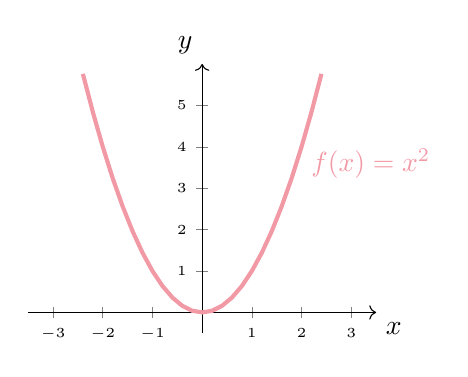
\begin{tikzpicture}
			\begin{axis}[
				clip=false,
				width=6cm, height=5cm,
				xmin=-3.5, xmax=3.5, ymin=-0.5, ymax=6,
				xtick={-3,-2,-1,0,1,2,3},
				ytick={1,2,3,4,5},
				axis lines=middle, axis line style={->},
				xlabel={$x$}, ylabel={$y$},
				xlabel style={below right}, ylabel style={above left},
				tick label style={font=\tiny},
			]
			\addplot[color=pink!80!purple, line width=1.5pt, domain=-2.4:2.4] {x^2};
			\node[above right, pink!80!purple] at (2, 3) {$f(x)=x^2$};
			\end{axis}
		\end{tikzpicture}
		\column{0.48\textwidth}
		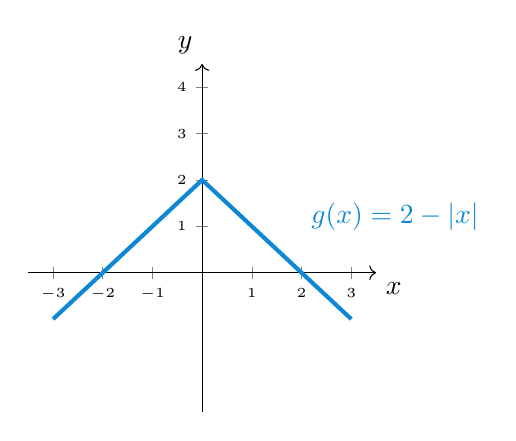
\begin{tikzpicture}
			\begin{axis}[
				clip=false,
				width=6cm, height=6cm,
				xmin=-3.5, xmax=3.5, ymin=-3, ymax=4.5,
				xtick={-3,-2,-1,0,1,2,3},
				ytick={1,2,3,4,5},
				axis lines=middle, axis line style={->},
				xlabel={$x$}, ylabel={$y$},
				xlabel style={below right}, ylabel style={above left},
				tick label style={font=\tiny},
			]
			\addplot[color=cyan!70!blue, line width=1.5pt, domain=-3:3] {2-abs(x)};
			\node[right, cyan!70!blue] at (2, 1.2) {$g(x)=2-|x|$};
			\end{axis}
		\end{tikzpicture}
	\end{columns}
	\begin{summarybox-answer}
	这两个函数的图象都关于 \(\boldsymbol{y}\) 轴\textbf{对称}.
	\end{summarybox-answer}
\end{frame}

\begin{frame}{探究：自变量取相反数，函数值相等}
	\begin{exploration}
	取自变量的一些特殊值，观察相应函数值的情况：
	\end{exploration}
	\begin{center}
		\renewcommand{\arraystretch}{1.3}
		\begin{tabular}{|c|c|c|c|c|c|c|c|}
			\hline
			\(x\) & \(\cdots\) & \(-2\) & \(-1\) & \(0\) & \(1\) & \(2\) & \(\cdots\) \\ \hline
			\(f(x)=x^2\) & \(\cdots\) & \(4\) & \(1\) & \(0\) & \(1\) & \(4\) & \(\cdots\) \\ \hline
			\(g(x)=2-|x|\) & \(\cdots\) & \(0\) & \(1\) & \(2\) & \(1\) & \(0\) & \(\cdots\) \\ \hline
		\end{tabular}
	\end{center}
	\pause
	\begin{summarybox-answer}
	当自变量取一对相反数时，相应的两个函数值\textbf{相等}. 例如 \(f(-2)=4=f(2)\)，\(f(-1)=1=f(1)\).\\
	事实上，\(\forall x\in\mathbf{R}\)，都有 \(f(-x)=(-x)^2=x^2=f(x)\).
	\end{summarybox-answer}
\end{frame}

\begin{frame}{偶函数的定义}
	\begin{summarybox}[偶函数（even function）]
	一般地，设函数 \(f(x)\) 的定义域为 \(D\)，如果 \(\forall x\in D\)，都有 \(-x\in D\)，且
	\[
		f(-x)=f(x),
	\]
	那么函数 \(f(x)\) 就叫做\textbf{偶函数}.
	\end{summarybox}
	\vspace{0.5em}
	\begin{summarybox-answer}
	\textbf{两个要点}：\\
	① 定义域关于原点对称（\(x\in D\Rightarrow -x\in D\)）；\\
	② \(f(-x)=f(x)\).\\[3pt]
	\textbf{图象特征}：偶函数的图象关于 \(y\) 轴对称.
	\end{summarybox-answer}
\end{frame}

\begin{frame}{例：偶函数 \(f(x)=x^2+1\) 的图象}
	\begin{columns}
		\column{0.45\textwidth}
		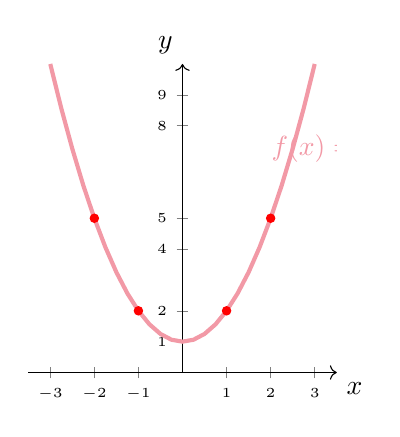
\begin{tikzpicture}[baseline=(current bounding box.north)]
			\begin{axis}[
				width=5.5cm, height=5.5cm,
				xmin=-3.5, xmax=3.5, ymin=0, ymax=10,
				xtick={-3,-2,-1,0,1,2,3},
				ytick={1,2,4,5,8,9},
				axis lines=middle, axis line style={->},
				xlabel={$x$}, ylabel={$y$},
				xlabel style={below right}, ylabel style={above left},
				tick label style={font=\tiny},
			]
			\addplot[color=pink!80!purple, line width=1.5pt, domain=-3:3] {x^2+1};
			\addplot[only marks, mark=*, mark size=1.5pt, color=red] coordinates {(1,2) (-1,2) (2,5) (-2,5)};
			\node[above right, pink!80!purple] at (1.8, 6.5) {$f(x)=x^2+1$};
			\end{axis}
		\end{tikzpicture}
		\column{0.55\textwidth}
		\vspace{1em}
		\begin{summarybox-answer}
		\(f(-x)=(-x)^2+1=x^2+1=f(x)\)，是偶函数.\\[4pt]
		点 \((1,2)\) 与 \((-1,2)\)、\((2,5)\) 与 \((-2,5)\) 都关于 \(y\) 轴对称.
		\end{summarybox-answer}
	\end{columns}
\end{frame}

\section{奇函数}

\begin{frame}{探究：\(f(x)=x\) 与 \(g(x)=\dfrac{1}{x}\) 的图象}
	观察函数 \(f(x)=x\) 和 \(g(x)=\dfrac{1}{x}\) 的图象，它们有什么共同特征？
	\begin{columns}
		\column{0.48\textwidth}
		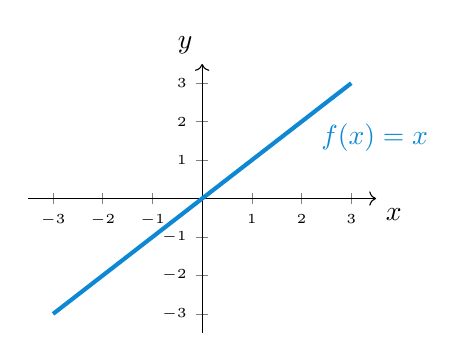
\begin{tikzpicture}
			\begin{axis}[
				clip=false,
				width=6cm, height=5cm,
				xmin=-3.5, xmax=3.5, ymin=-3.5, ymax=3.5,
				xtick={-3,-2,-1,0,1,2,3},
				ytick={-3,-2,-1,1,2,3},
				axis lines=middle, axis line style={->},
				xlabel={$x$}, ylabel={$y$},
				xlabel style={below right}, ylabel style={above left},
				tick label style={font=\tiny},
			]
			\addplot[color=cyan!70!blue, line width=1.5pt, domain=-3:3] {x};
			\node[below right, cyan!70!blue] at (2.2, 2.2) {$f(x)=x$};
			\end{axis}
		\end{tikzpicture}
		\column{0.48\textwidth}
		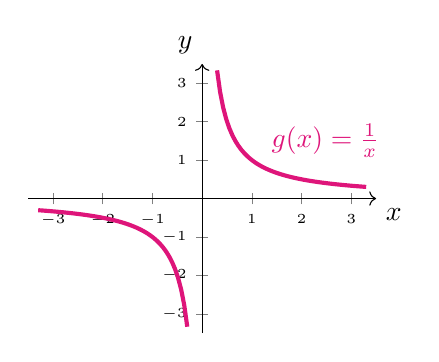
\begin{tikzpicture}
			\begin{axis}[
				width=6cm, height=5cm,
				xmin=-3.5, xmax=3.5, ymin=-3.5, ymax=3.5,
				xtick={-3,-2,-1,1,2,3},
				ytick={-3,-2,-1,1,2,3},
				axis lines=middle, axis line style={->},
				xlabel={$x$}, ylabel={$y$},
				xlabel style={below right}, ylabel style={above left},
				tick label style={font=\tiny},
			]
			\addplot[domain=-3.3:-0.3, color=magenta!70!purple, line width=1.5pt, samples=50] {1/x};
			\addplot[domain=0.3:3.3, color=magenta!70!purple, line width=1.5pt, samples=50] {1/x};
			\node[right, magenta!70!purple] at (1.2, 1.5) {$g(x)=\frac{1}{x}$};
			\end{axis}
		\end{tikzpicture}
	\end{columns}
	\begin{summarybox-answer}
	两个函数的图象都关于原点成中心对称图形.
	\end{summarybox-answer}
\end{frame}

\begin{frame}{奇函数的定义}
	当自变量取一对相反数时，相应的函数值也是一对相反数. 如 \(f(x)=x\)：\(f(-3)=-3=-f(3)\)，\(f(-2)=-2=-f(2)\).
	\begin{summarybox}[奇函数（odd function）]
	一般地，设函数 \(f(x)\) 的定义域为 \(D\)，如果 \(\forall x\in D\)，都有 \(-x\in D\)，且
	\[
		f(-x)=-f(x),
	\]
	那么函数 \(f(x)\) 就叫做\textbf{奇函数}.
	\end{summarybox}
	\vspace{0.3em}
	\begin{summarybox-answer}
	\textbf{图象特征}：奇函数的图象关于\textbf{原点}对称.
	\end{summarybox-answer}
\end{frame}

\section{奇偶性的判断}

\begin{frame}{例6：判断下列函数的奇偶性}
	\setcounter{exam}{5}
	\begin{exam}
	判断下列函数的奇偶性：\\
	(1) \(f(x)=x^4\)；\qquad\qquad(2) \(f(x)=x^5\)；\\
	(3) \(f(x)=x+\dfrac{1}{x}\)；\qquad (4) \(f(x)=\dfrac{1}{x^2}\).
	\end{exam}
	\vspace{0.3em}
%	\begin{summarybox-answer}
%	\textbf{注意}：奇偶性是函数在它的定义域上的\textbf{整体性质}，所以判断奇偶性应先明确它的\textbf{定义域}.
%	\end{summarybox-answer}
\end{frame}

\begin{frame}{例6（1）（2）}
	\begin{solve}
	(1) \(f(x)=x^4\) 的定义域为 \(\mathbf{R}\). 因为 \(\forall x\in\mathbf{R}\)，都有 \(-x\in\mathbf{R}\)，且
	\[
		f(-x)=(-x)^4=x^4=f(x),
	\]
	所以 \(f(x)=x^4\) 为\textbf{偶函数}.
	\end{solve}
	\vspace{0.3em}
	\pause
	\begin{solve}
	(2) \(f(x)=x^5\) 的定义域为 \(\mathbf{R}\). 且
	\[
		f(-x)=(-x)^5=-x^5=-f(x),
	\]
	所以 \(f(x)=x^5\) 为\textbf{奇函数}.
	\end{solve}
\end{frame}

\begin{frame}{例6（3）（4）：分式函数}\vspace{-1.5em}
	\begin{solve}
	(3) \(f(x)=x+\dfrac{1}{x}\) 的定义域为 \(\{x\mid x\neq 0\}\). 且
	\[
		f(-x)=-x+\frac{1}{-x}=-\Bigl(x+\frac{1}{x}\Bigr)=-f(x),
	\]
	所以 \(f(x)=x+\dfrac{1}{x}\) 为\textbf{奇函数}.
	\end{solve}
	\vspace{-1em}
	\pause
	\begin{solve}
	(4) \(f(x)=\dfrac{1}{x^2}\) 的定义域为 \(\{x\mid x\neq 0\}\). 且
	\[
		f(-x)=\frac{1}{(-x)^2}=\frac{1}{x^2}=f(x),
	\]
	所以 \(f(x)=\dfrac{1}{x^2}\) 为\textbf{偶函数}.
	\end{solve}
\end{frame}

%\begin{frame}{}
%	\begin{columns}
%		\column{0.50\textwidth}
%		\begin{tikzpicture}[baseline=(current bounding box.north)]
%			\begin{axis}[
%				clip=false,
%				width=5.5cm, height=5.5cm,
%				xmin=-2.2, xmax=2.2, ymin=-8.5, ymax=8.5,
%				xtick={-2,-1,0,1,2},
%				ytick={-8,-2,2,8},
%				axis lines=middle, axis line style={->},
%				xlabel={$x$}, ylabel={$y$},
%				xlabel style={below right}, ylabel style={above left},
%				tick label style={font=\small},
%			]
%			\addplot[color=green!50!black, line width=1.5pt, domain=-2:2] {x^3+x};
%%			\addplot[only marks, mark=*, mark size=1.5pt, color=red] coordinates {(1,1) (-1,-1)};
%			\node[right, green!50!black,anchor=west] at (1.8, 4) {$f(x)=x^3+x$};
%			\end{axis}
%		\end{tikzpicture}
%		\column{5\textwidth}
%		\vspace{2em}\hspace{-2em}
%		\begin{summarybox-answer}
%		\(f(-x)=(-x)^3=-x^3=-f(x)\)，是奇函数.\\[4pt]
%		点 \((1,1)\) 与 \((-1,-1)\) 关于\textbf{原点}对称.
%		\end{summarybox-answer}
%	\end{columns}
%\end{frame}

\begin{frame}{思考：利用对称性简化研究}\vspace{-2em}
	\begin{summarybox}
	\begin{enumerate}[(1)]
		\item 判断函数 \(f(x)=x^3+x\) 的奇偶性.
		\item 图是函数$f(x)=x^3+x$图象的一部分，你能根据$f(x)$的奇偶性画出它在$y$轴左边的图象吗？
		\item 如果知道 \(y=f(x)\) 是偶（奇）函数，那么可以怎样简化对它的研究？
	\end{enumerate}
	\end{summarybox}
	\vspace{-2em}
	\begin{center}
	\begin{tikzpicture}[baseline=(current bounding box.north)]
		\begin{axis}[
			clip=false,
			width=5.5cm, height=5.5cm,
			xmin=-2.2, xmax=2.2, ymin=-8.5, ymax=8.5,
			xtick={-2,-1,0,1,2},
			ytick={-8,-2,2,8},
			axis lines=middle, axis line style={->},
			xlabel={$x$}, ylabel={$y$},
			xlabel style={below right}, ylabel style={above left},
			tick label style={font=\small},
			]
			\addplot[color=green!50!black, line width=1.5pt, domain=0:2] {x^3+x};
			%			\addplot[only marks, mark=*, mark size=1.5pt, color=red] coordinates {(1,1) (-1,-1)};
			\node[right, green!50!black,anchor=west] at (1.8, 4) {$f(x)=x^3+x$};
		\end{axis}
	\end{tikzpicture}
\end{center}
\end{frame}

\begin{frame}
	\begin{summarybox-answer}
		(1) \(f(-x)=(-x)^3+(-x)=-x^3-x=-(x^3+x)=-f(x)\)，故为\textbf{奇函数}.\\[4pt]
		(2) $f(x) = x^3 + x$在$x<0$的图象如下图所示。\\[4pt]
		(3) 偶函数只需研究 \(y\) 轴一侧，奇函数只需研究原点一侧，另一侧由对称性即可得到.
	\end{summarybox-answer}
		\begin{center}\vspace{-2em}
		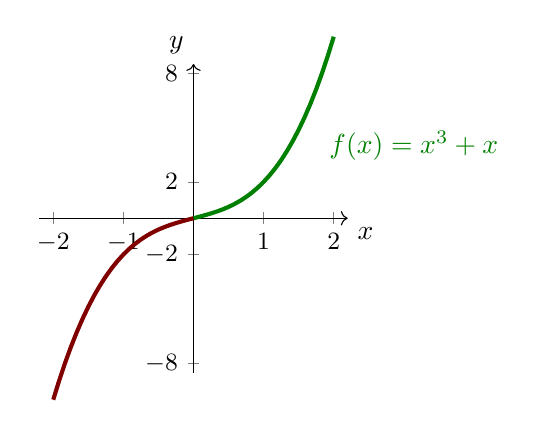
\begin{tikzpicture}[baseline=(current bounding box.north)]
			\begin{axis}[
				clip=false,
				width=5.5cm, height=5.5cm,
				xmin=-2.2, xmax=2.2, ymin=-8.5, ymax=8.5,
				xtick={-2,-1,0,1,2},
				ytick={-8,-2,2,8},
				axis lines=middle, axis line style={->},
				xlabel={$x$}, ylabel={$y$},
				xlabel style={below right}, ylabel style={above left},
				tick label style={font=\small},
				]
				\addplot[color=green!50!black, line width=1.5pt, domain=0:2] {x^3+x};
				\addplot[color=red!50!black, line width=1.5pt, domain=-2:0] {x^3+x};
				%			\addplot[only marks, mark=*, mark size=1.5pt, color=red] coordinates {(1,1) (-1,-1)};
				\node[right, green!50!black,anchor=west] at (1.8, 4) {$f(x)=x^3+x$};
			\end{axis}
		\end{tikzpicture}
	\end{center}
\end{frame}

\begin{frame}{布置作业}
	\begin{summarybox}[课后作业]
		\begin{enumerate}
			\item 教材 P85 练习 1、2、3
			\item P85-87习题3.2 ：5、12、13
		\end{enumerate}
	\end{summarybox}
\end{frame}

\section{课堂练习}

\begin{frame}{练习 1：判断下列函数的奇偶性}
	\begin{exercise}
	判断下列函数的奇偶性：\\
	(1) \(f(x)=2x^4+3x^2\)；\qquad (2) \(f(x)=x^3-2x\).
	\end{exercise}
	\pause
	\begin{solve}
	(1) \(f(-x)=2(-x)^4+3(-x)^2=2x^4+3x^2=f(x)\)，故为\textbf{偶函数}.\\[4pt]
	(2) \(f(-x)=(-x)^3-2(-x)=-x^3+2x=-(x^3-2x)=-f(x)\)，故为\textbf{奇函数}.
	\end{solve}
\end{frame}

\begin{frame}{练习 2：由对称性补全图象}
	\begin{exercise}
	已知 \(f(x)\) 是偶函数，\(g(x)\) 是奇函数，试根据它们在 \(y\) 轴一侧（或原点一侧）的图象，补全另一部分图象.
	\end{exercise}
			\begin{center}\vspace{-1em}
		\begin{tikzpicture}[baseline=(current bounding box.north)]
			\begin{axis}[
				clip=false,
				width=5.5cm, height=5.5cm,
				xmin=-2.2, xmax=2.2, ymin=-4.5, ymax=4.5,
				xtick={-2,-1,0,1,2},
				ytick={-8,-2,2,8},
				axis lines=middle, axis line style={->},
				xlabel={$x$}, ylabel={$y$},
				xlabel style={below right}, ylabel style={above left},
				tick label style={font=\small},
				]
				\begin{scope}
					\clip (-2.2,-4) rectangle (2.2,4);
					\draw [magenta,thick](0,0) .. controls (0.5,4) and (0.8,-1)  .. (2.0,1.8);
				\end{scope}
				\node[above] at (2.0,1.8) {$f(x)$};
			\end{axis}
		\end{tikzpicture}
		\hspace{2em}\begin{tikzpicture}[baseline=(current bounding box.north)]
			\begin{axis}[
				clip=false,
				width=5.5cm, height=5.5cm,
				xmin=-2.2, xmax=2.2, ymin=-4.5, ymax=4.5,
				xtick={-2,-1,0,1,2},
				ytick={-8,-2,2,8},
				axis lines=middle, axis line style={->},
				xlabel={$x$}, ylabel={$y$},
				xlabel style={below right}, ylabel style={above left},
				tick label style={font=\small},
				]
				\begin{scope}
					\clip (-2.2,-4) rectangle (2.2,4);
					\draw [magenta,thick](0,0) .. controls (0.5,4) and (0.8,-1)  .. (2.0,1.8);
				\end{scope}
				\node[above] at (2.0,1.8) {$g(x)$};
			\end{axis}
		\end{tikzpicture}
		\end{center}
	
\end{frame}

\begin{frame}
	
	\begin{summarybox-answer}
		\textbf{方法}：\\
		· 偶函数：把 \(y\) 轴右侧的图象沿 \(y\) 轴\textbf{翻折}到左侧；\\
		· 奇函数：把已知部分的图象绕原点\textbf{旋转 \(180^\circ\)}，得到另一部分.
	\end{summarybox-answer}
		\begin{center}\vspace{-1em}
		\begin{tikzpicture}[baseline=(current bounding box.north)]
			\begin{axis}[
				clip=false,
				width=5.5cm, height=5.5cm,
				xmin=-2.2, xmax=2.2, ymin=-4.5, ymax=4.5,
				xtick={-2,-1,0,1,2},
				ytick={-8,-2,2,8},
				axis lines=middle, axis line style={->},
				xlabel={$x$}, ylabel={$y$},
				xlabel style={below right}, ylabel style={above left},
				tick label style={font=\small},
				]
				\begin{scope}
					\clip (-2.2,-4) rectangle (2.2,4);
					\draw [magenta,thick](0,0) .. controls (0.5,4) and (0.8,-1)  .. (2.0,1.8);
					\draw [blue,thick](0,0) .. controls (-0.5,4) and (-0.8,-1)  .. (-2.0,1.8);
				\end{scope}
				\node[above] at (2.0,1.8) {$f(x)$};
			\end{axis}
		\end{tikzpicture}
		\hspace{2em}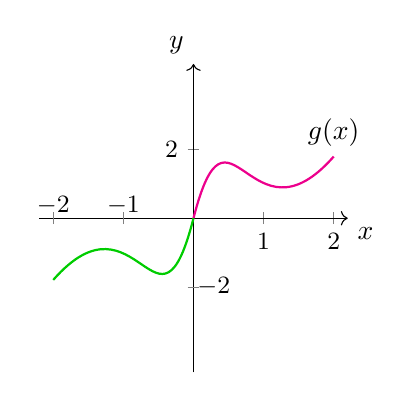
\begin{tikzpicture}[baseline=(current bounding box.north)]
			\begin{axis}[
				clip=false,
				width=5.5cm, height=5.5cm,
				xmin=-2.2, xmax=2.2, ymin=-4.5, ymax=4.5,
				xtick={0,1,2},
				ytick={2,8},
				extra x ticks={-2,-1},
				extra x tick style={xticklabel style={above}},
				extra y ticks={-2},
				extra y tick style={yticklabel style={right}},
				axis lines=middle, axis line style={->},
				xlabel={$x$}, ylabel={$y$},
				xlabel style={below right}, ylabel style={above left},
				tick label style={font=\small},
				]
				\begin{scope}
					\clip (-2.2,-4) rectangle (2.2,4);
					\draw [magenta,thick](0,0) .. controls (0.5,4) and (0.8,-1)  .. (2.0,1.8);
					\draw [green!80!black,thick,rotate around={180:(0,0)}](0,0) .. controls (0.5,4) and (0.8,-1)  .. (2.0,1.8);
				\end{scope}
				\node[above] at (2.0,1.8) {$g(x)$};
			\end{axis}
		\end{tikzpicture}
	\end{center}
\end{frame}

\begin{frame}
	\begin{exercise}
		\begin{enumerate}[(1)]
			\item 从偶函数的定义出发，证明函数$y=f(x)$是偶函数的充要条件是它的图象关于$y$轴对称；
			\item 从奇函数的定义出发，证明函数$y=f(x)$是奇函数的充要条件是它的图象关于原点对称；
		\end{enumerate}
		
	\end{exercise}
\end{frame}

\begin{frame}
	\begin{prooft}
		1.	（1）充分性:
		若函数 $y=f(x)$ 的图象关于 $y$ 轴对称。
		在函数图象上任取一点 $P(x, f(x))$。
		因为图象关于 $y$ 轴对称，所以点 $P$ 关于 $y$ 轴的对称点 $P\,'(-x, f(x))$ 也一定在函数图象上。
		根据函数图象上点的坐标特征，点 $P\,'$ 的坐标也可以表示为 $(-x, f(-x))$。
		因此，两点的纵坐标相等，即：
		$$f(-x) = f(x)$$
		又因为图象关于 $y$ 轴对称，所以函数的定义域关于原点对称。
		满足偶函数的定义，所以函数 $y=f(x)$ 是偶函数。
		
	\end{prooft}
\end{frame}

\begin{frame}
	\begin{prooft}
		
	(2)	必要性:
		假设函数 $y=f(x)$ 是偶函数。
		根据偶函数的定义，对于定义域内的任意 $x$，都有 $f(-x) = f(x)$，且定义域关于原点对称。
		在函数图象上任取一点 $P(x_0, y_0)$，则有 $y_0 = f(x_0)$。
		考察点 $P$ 关于 $y$ 轴的对称点 $P\,'(-x_0, y_0)$。
		因为定义域关于原点对称，所以 $-x_0$ 也在定义域内。
		将 $-x_0$ 代入函数解析式，由于 $f(x)$ 是偶函数，可得：
		$$f(-x_0) = f(x_0) = y_0$$
		这说明点 $P\,^\prime(-x_0, y_0)$ 的坐标满足函数关系式，即点 $P\,'$ 也在函数 $y=f(x)$ 的图象上。
		因为图象上任意一点关于 $y$ 轴的对称点都在图象上，所以函数 $y=f(x)$ 的图象关于 $y$ 轴对称。
		
		
		综上所述，函数 $y=f(x)$ 是偶函数的充要条件是它的图象关于 $y$ 轴对称。
	\end{prooft}
\end{frame}

\begin{frame}
	\begin{prooft}
		2（1）充分性:
		若函数 $y=f(x)$ 的图象关于原点对称。
		在函数图象上任取一点 $P(x, f(x))$。
		因为图象关于原点对称，所以点 $P$ 关于原点的对称点 $P\,'(-x, -f(x))$ 也一定在函数图象上。
		根据函数图象上点的坐标特征，点 $P\,'$ 的坐标也可以表示为 $(-x, f(-x))$。
		因此，两点的纵坐标相等，即：
		$$f(-x) = -f(x)$$
		又因为图象关于原点对称，所以函数的定义域关于原点对称。
		满足奇函数的定义，所以函数 $y=f(x)$ 是奇函数。
	\end{prooft}
\end{frame}

\begin{frame}
	\begin{prooft}	
	（2）必要性:
	若函数 $y=f(x)$ 是奇函数。
	根据奇函数的定义，对于定义域内的任意 $x$，都有 $f(-x) = -f(x)$，且定义域关于原点对称。
	在函数图象上任取一点 $P(x_0, y_0)$，则有 $y_0 = f(x_0)$。
	考察点 $P$ 关于原点的对称点 $P\,'(-x_0, -y_0)$。
	因为定义域关于原点对称，所以 $-x_0$ 也在定义域内。
	将 $-x_0$ 代入函数解析式，由于 $f(x)$ 是奇函数，可得：
	$$f(-x_0) = -f(x_0) = -y_0$$
	这说明点 $P\,'(-x_0, -y_0)$ 的坐标满足函数关系式，即点 $P\,'$ 也在函数 $y=f(x)$ 的图象上。
	因为图象上任意一点关于原点的对称点都在图象上，所以函数 $y=f(x)$ 的图象关于原点对称。
	
	
	综上所述，函数 $y=f(x)$ 是奇函数的充要条件是它的图象关于原点对称。
	\end{prooft}
\end{frame}
	

\end{document}
